\clearpage % Start a new page
\lhead{\emph{Propuesta de experimentación
numérica}}
\chapter{Propuesta de experimentación
numérica}
\label{sec:Propuesta de experimentación
numérica}

En este capítulo se describe detalladamente el diseño experimental empleado para evaluar y comparar modelos de predicción del nivel del río Paraguay. Primero, se presenta el entorno computacional utilizado, incluyendo hardware y software. A continuación, se caracterizan los datos y la instancia del problema, especificando las variables consideradas y el período de estudio. Luego se expone el flujo completo de la experimentación, definiendo los pasos de preprocesamiento, partición temporal, ajuste de hiperparámetros y configuración de los distintos experimentos. Finalmente, se introducen las métricas de evaluación que se emplearán para cuantificar el desempeño de cada modelo, así como los horizontes de pronóstico analizados.
\section{Ambiente computacional}
\label{sec:ambiente_computacional}

\subsection{Hardware}
\label{ssec:hardware}

En la Tabla \ref{tab:hardware} se presentan las especificaciones de hardware utilizadas para ejecutar los experimentos:

\begin{table}[h]
  \centering
  \caption{Especificaciones de hardware}
  \label{tab:hardware}
  \begin{tabular}{@{}ll@{}}
    \toprule
    \textbf{Componente} & \textbf{Detalle} \\
    \midrule
    Placa madre         & MSI PRO Z690-A WIFI DDR4 \\
    Procesador          & 12th Gen Intel Core i5-12400F \\
    Memoria RAM         & 32\,GB DDR4 \\
    Almacenamiento      & SSD 500 GB A3N SanDisk \\
    Tarjeta gráfica     & NVIDIA GeForce RTX 3060 Ti \\
    \bottomrule
  \end{tabular}
\end{table}

\subsection{Software}
\label{ssec:software}

En la Tabla \ref{tab:software} se detallan las versiones de software empleadas en el desarrollo y entrenamiento de los modelos:

\begin{table}[h]
  \centering
  \caption{Versiones de software utilizadas}
  \label{tab:software}
  \begin{tabular}{@{}ll@{}}
    \toprule
    \textbf{Elemento}                   & \textbf{Versión / Detalle} \\
    \midrule
    Sistema operativo                   & Linux Mint 22 Wilma LTS \\
    Lenguaje de programación            & Python 3.10.6 \\
    Librería de aprendizaje profundo    & TensorFlow 2.12.0 \\
    Librería de búsqueda de hiperparámetros & Optuna 3.2 \\
    \bottomrule
  \end{tabular}
\end{table}


\section{Datos e instancia del problema}
\label{sec:datos_instancia}

\subsection{Fuentes y descripción del conjunto de datos}
\label{ssec:fuentes_datos}

El río Paraguay, el principal afluente del río Paraná, es el quinto río más grande de América del Sur, con una cuenca de drenaje que cubre aproximadamente 984.000 kilómetros cuadrados. Con una longitud de 2.549 kilómetros, el río nace en el estado de Mato Grosso, Brasil, y fluye hacia el sur a través de llanuras, humedales y pantanos. En Paraguay, continúa su curso hacia el sur, formando la frontera con Argentina en los últimos 240 kilómetros antes de desembocar en el río Paraná, que finalmente drena hacia el océano Atlántico
\cite{paraguayriverbritannica}. El caudal y los niveles de agua del río son fundamentales para la navegación, la agricultura y la planificación de infraestructuras en la región.
A lo largo del Río Paraguay existen puntos denominados estaciones, donde se miden y registran el nivel del río, las precipitaciones y los caudales. En la Fig.~\ref{fig:mapa_estaciones_paraguay} se muestran las seis estaciones utilizadas en este estudio. Los datos recopilados diariamente conforman lo que se conoce como series temporales.

\begin{figure}[]
    \begin{center}
        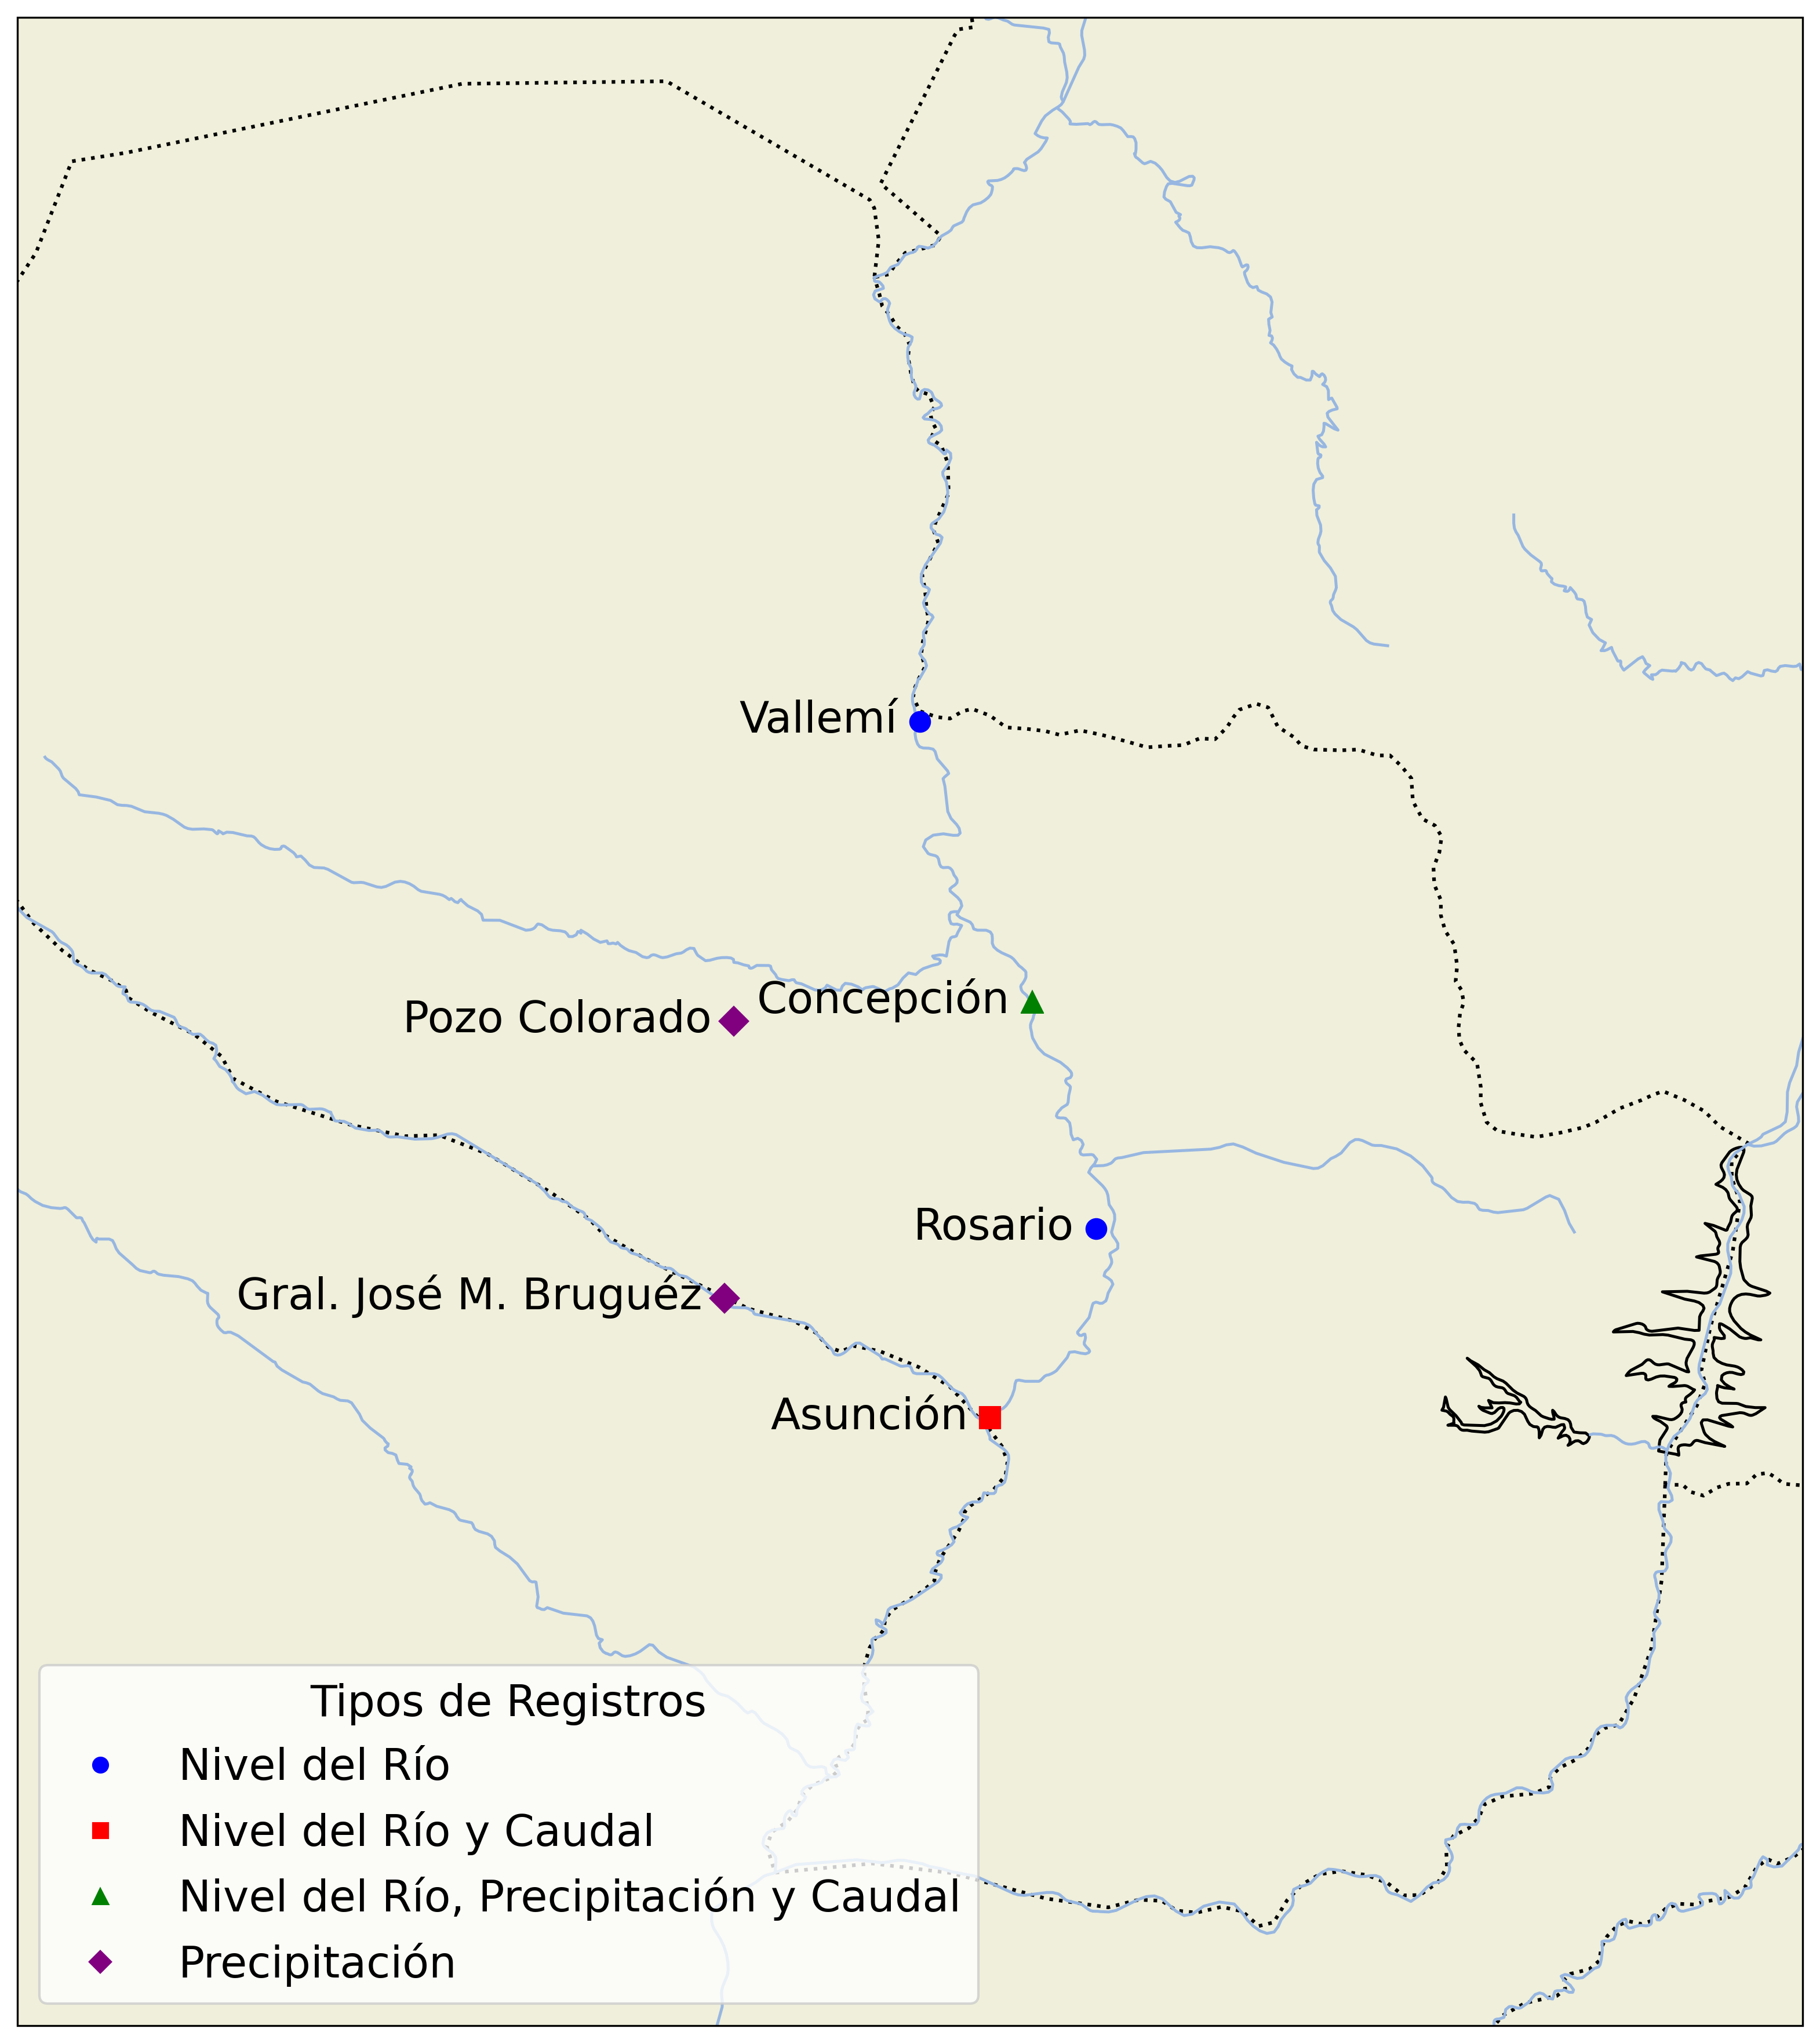
\includegraphics[width=13cm,height=15cm]{Figuras/mapa_estaciones_paraguay.png}
        \caption{Ubicación de las estaciones de medición utilizadas en el estudio.}
        \label{fig:mapa_estaciones_paraguay}
    \end{center}
\end{figure}

Los datos utilizados en este estudio fueron proporcionados por la División Meteorológica de la Facultad Politécnica de la Universidad Nacional de Asunción (FPUNA) y la Dirección Nacional de Aeronáutica Civil (DINAC). El foco principal de este estudio es la estación 86218, ubicada en el Puerto de Asunción, con registros de niveles de agua desde 1904. Además, se incorporaron datos de otras estaciones con registros desde 1970, incluyendo estaciones de precipitación en afluentes del río y datos de caudales de ríos, resultando en un conjunto de datos con registros diarios desde 1995 hasta finales del año 2022 para este estudio.

Para modelar la dinámica hidrológica se seleccionaron las siguientes variables de entrada:

\begin{itemize}
  \item \textbf{Nivel del río}: altura del agua registrada diariamente en cada estación.
  \item \textbf{Caudal}: volumen de agua que pasa por la sección de medición por unidad de tiempo.
  \item \textbf{Precipitación}: acumulado de lluvia diaria en las estaciones que lo registran.
\end{itemize}

A continuación se presentan los metadatos de las seis estaciones empleadas (Tabla \ref{tabla:informacion_estaciones}):

\begin{table}[h]
  \caption{Información de las estaciones de medición}
  \label{tabla:informacion_estaciones}
  \centering
  \renewcommand{\arraystretch}{1.3}
  \setlength{\tabcolsep}{2pt}
  \resizebox{\columnwidth}{!}{
    \begin{tabular}{|c|c|c|c|c|}
      \hline
      \textbf{Estación} & \textbf{Ciudad} & \textbf{Ubicación (Lat., Long.)} & \textbf{Variables registradas} & \textbf{Datos desde} \\ \hline
      86218 & Asunción                & -25.27, -57.64                     & Nivel del Río y Caudal            & 1904-01-02 \\ \hline
      86088 & Vallemí                 & -22.15, -57.95                     & Nivel del Río                     & 1971-07-21 \\ \hline
      86134 & Concepción             & -23.41, -57.45                     & Nivel del Río, Precipitación, Caudal & 1909-10-01 \\ \hline
      86183 & Rosario                 & -24.42, -57.16                     & Nivel del Río                     & 1932-01-01 \\ \hline
      86170 & Gral. José M. Bruguéz & -24.74, -58.83                     & Precipitación                     & 1992-01-01 \\ \hline
      86128 & Pozo Colorado           & -23.49, -58.79                     & Precipitación                     & 1995-01-01 \\ \hline
    \end{tabular}
  }
\end{table}

\subsection{Ingeniería de Características}
En el proceso de ingeniería de características, se generaron nuevas variables que representan acumulaciones móviles de precipitaciones a lo largo de ventanas temporales específicas, como se muestra en la Tabla~\ref{tabla:informacion_estaciones_derivadas}.
La inclusión de estas acumulaciones móviles demostró tener un impacto significativo en la mejora de la correlación con la estación objetivo y permitió obtener mejores desfases temporales (lags) en el análisis de correlación cruzada, como se puede ver en la Tabla~\ref{tabla:correlaciones_maximas}. Este análisis también se extendió a las demás covariables, lo que permitió identificar las variables con la mayor correlación y los desfases temporales (lags) más relevantes, como se muestra en la Fig.~\ref{fig:lags}.

Aunque no se incorporaron desfases temporales como nuevas variables, el análisis de correlación cruzada entre las covariables y la variable objetivo ayudó a identificar las relaciones temporales significativas. Esto permitió comprender cómo las precipitaciones acumuladas y otras covariables influyen en los niveles de agua, mejorando así la precisión de las predicciones. Además, los lags obtenidos sirvieron como referencia para definir la ventana de búsqueda utilizada en la generación de acumulaciones móviles de precipitaciones.

\begin{figure}
    \centering
    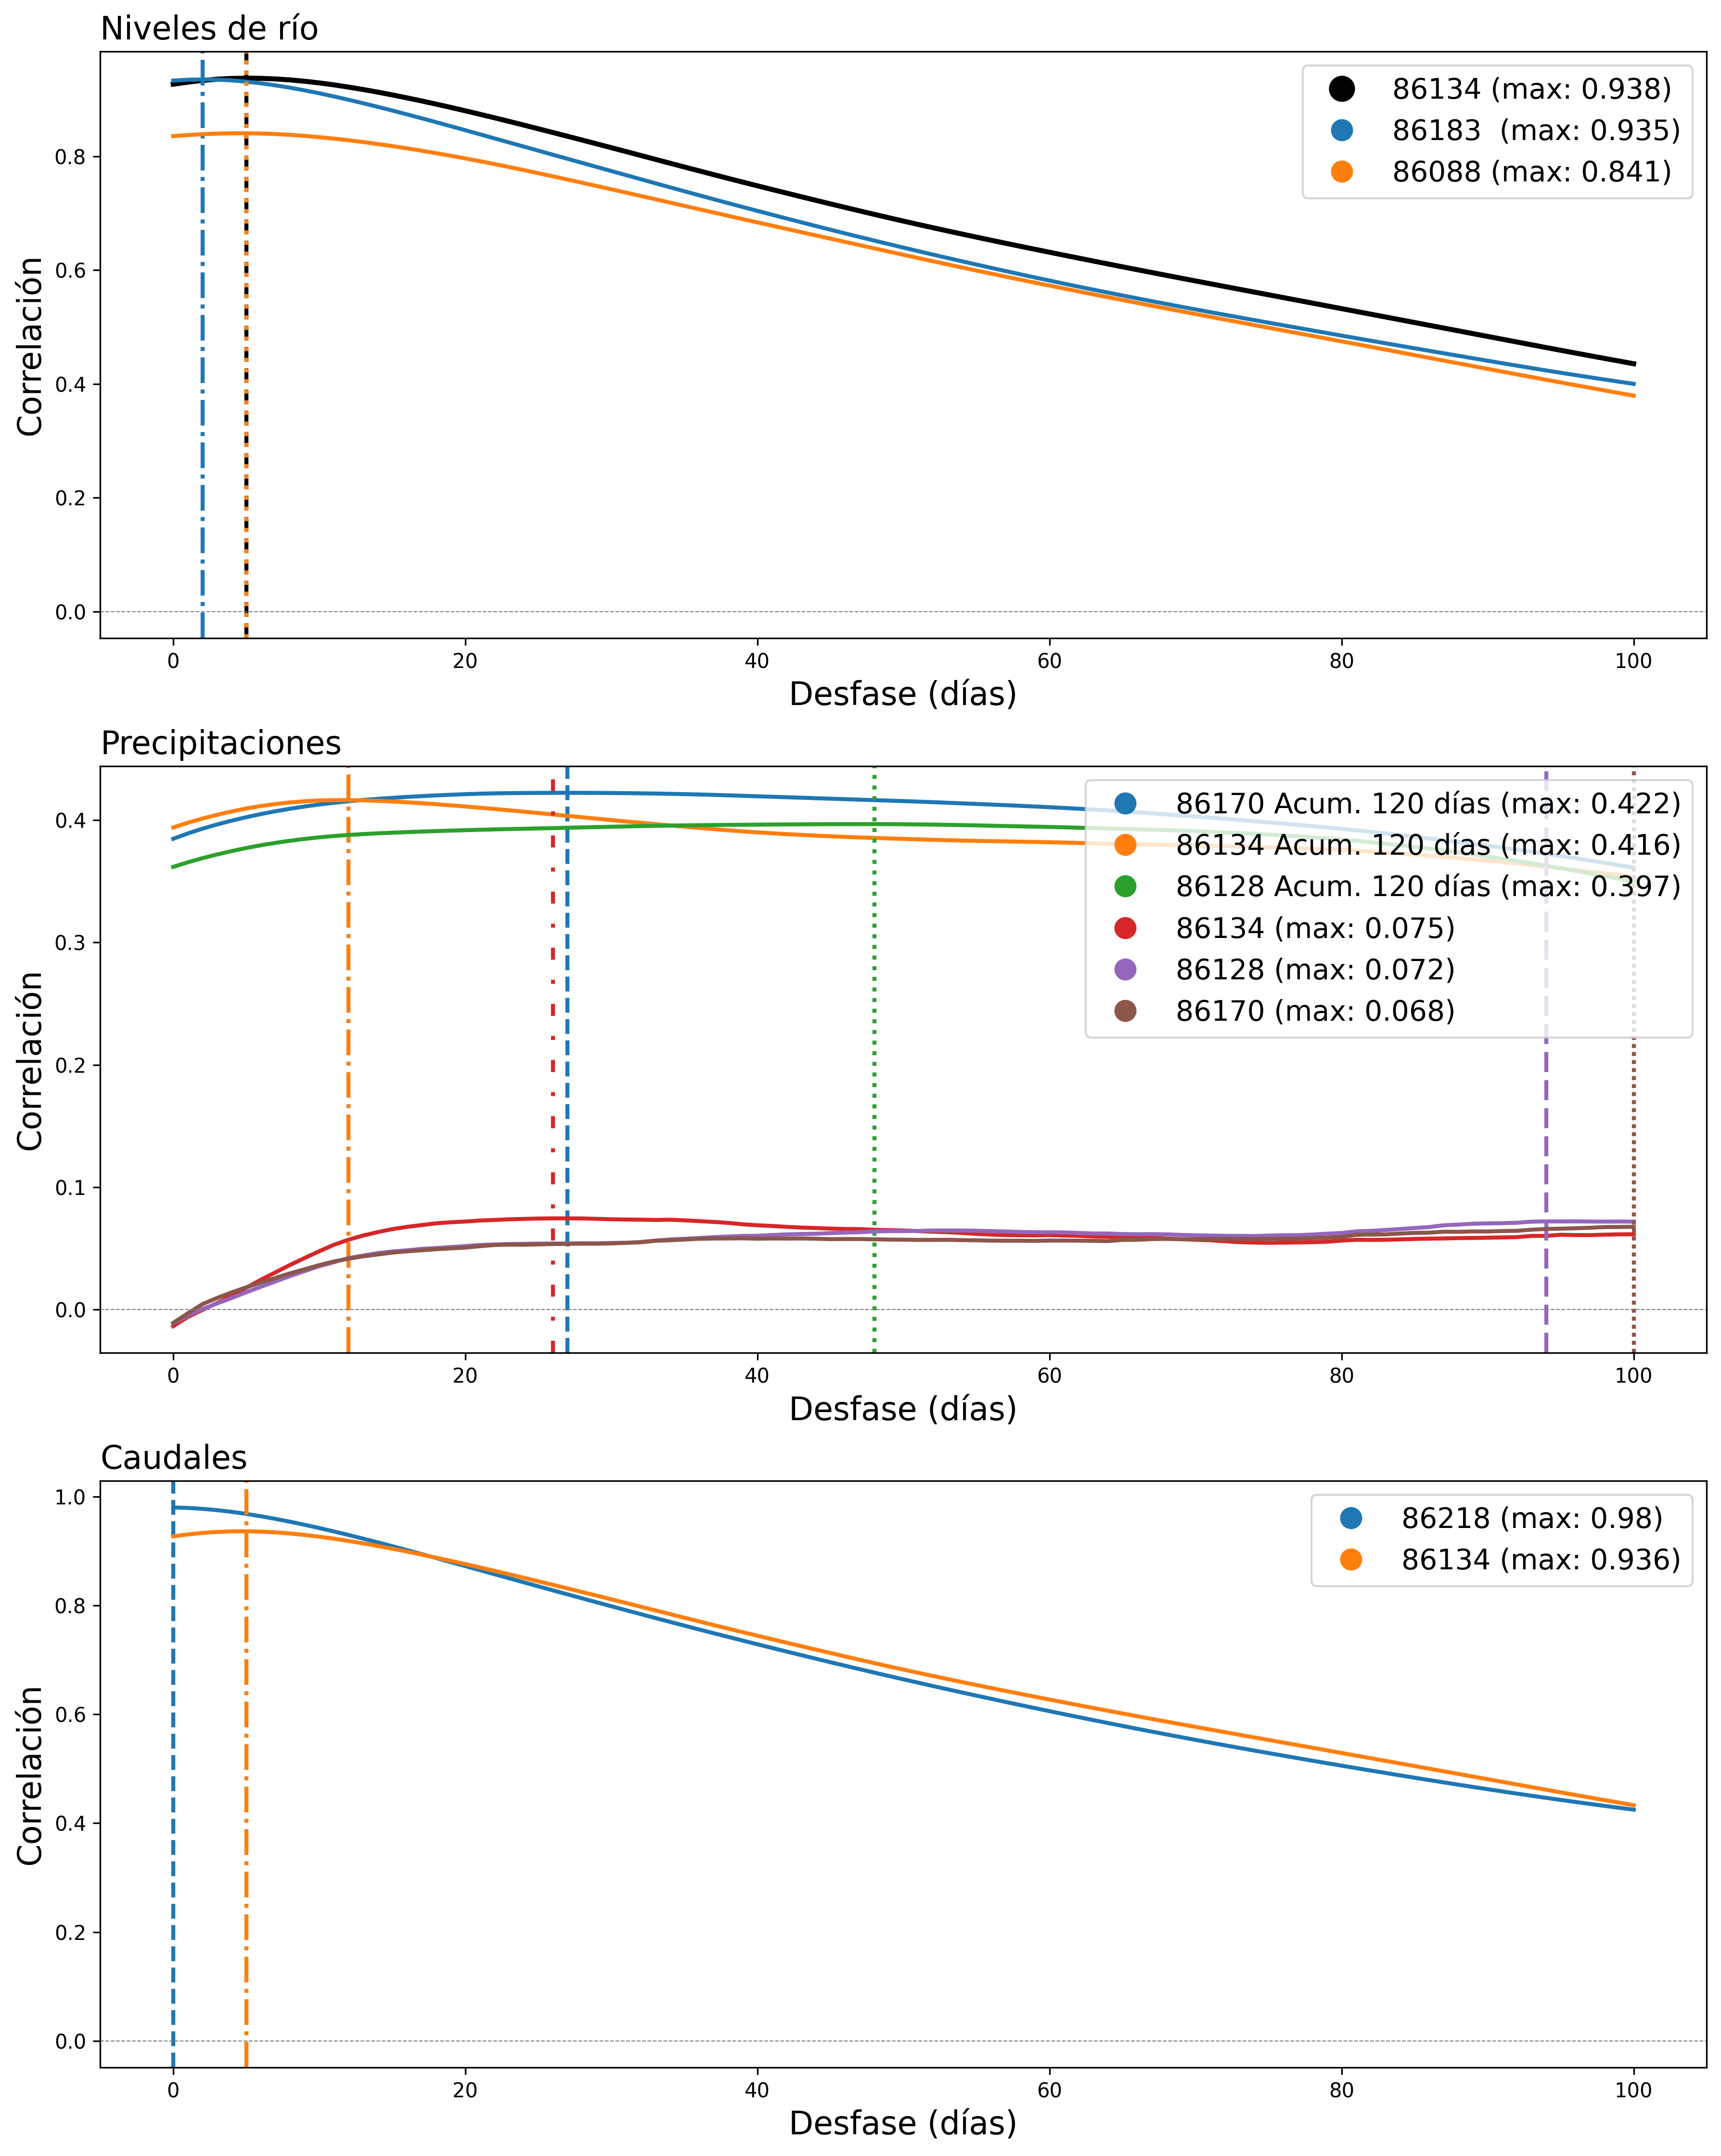
\includegraphics[width=1\linewidth,height=7.5cm]{Figuras/correlacion_cruzada_todo_en_uno.png}
    \caption{Correlaciones cruzadas máximas entre la estación objetivo (86218 - Asunción) y otras estaciones, agrupadas por tipo de variable: niveles, precipitaciones y caudales.Todas las series fueron previamente normalizadas utilizando Min-Max.}
    \label{fig:lags}
\end{figure}

\begin{table}[!t]
  \caption{Caracteristicas derivadas a partir de los registros de precipitación} 
    \centering
    
    \renewcommand{\arraystretch}{1.3} % Altura de las filas
    \setlength{\tabcolsep}{3pt} % Espaciado entre columnas
    \resizebox{\columnwidth}{!}{ % Ajusta la tabla al ancho de una columna
    \begin{tabular}{|c|c|c|c|c|}
        \hline
        \textbf{Estación} & \textbf{Ciudad} & \textbf{Ubicación (Lat., Long.)} & \textbf{Registros de} & \textbf{Datos desde}  \\ \hline
        86134 & Concepción & -23.41, -57.45 & Precipitación acumulada 2 días & 1909-10-01 \\ \hline
        86170 & Gral. José M. Bruguéz & -24.74, -58.83 & Precipitación acumulada 170 días& 1992-01-01 \\ \hline
        86128 & Pozo Colorado & -23.49, -58.79 & Precipitación acumulada 215 días & 1995-01-01 \\ \hline
    \end{tabular}
    }
    \vspace{0.5cm} 
  
    \label{tabla:informacion_estaciones_derivadas}
\end{table}

\begin{table}[!t]
  \caption{Resumen de correlaciones máximas entre la estación objetivo (86218) Asunción y las variables independientes} 
  \centering

  \renewcommand{\arraystretch}{1.3} % Altura de las filas
  \setlength{\tabcolsep}{3pt} % Espaciado entre columnas
  \resizebox{\columnwidth}{!}{ % Ajusta la tabla al ancho de una columna
  \begin{tabular}{|c|c|c|c|c|}
    \hline
    \textbf{Estación} & \textbf{Ciudad} & \textbf{Variable} & \textbf{Corr. máx} & \textbf{Lag (días)} \\
    \hline
    86218 & Asunción & Caudal & 0.980 & 0 \\   \hline
    86134 & Concepción & Nivel & 0.937 & 5 \\   \hline
    86134 & Concepción & Caudal & 0.935 & 5 \\   \hline
    86183 & Rosario & Nivel & 0.934 & 2 \\   \hline
    86088 & Vallemí & Nivel & 0.840 & 5 \\   \hline
    86170 & Gral. José M. Bruguéz & Prec. acum. (120 días) & 0.429  & 25 \\   \hline
    86134 & Concepción & Prec. acum. (120 días) & 0.419  & 12 \\   \hline
    86128 & Pozo Colorado & Prec. acum. (120 días) & 0.393  & 41 \\   \hline
    86134 & Concepción & Precipitación diaria & 0.099 & 26 \\   \hline
    86128 & Pozo Colorado & Precipitación diaria & 0.071 & 94 \\   \hline
    86170 & Gral. José M. Bruguéz & Precipitación diaria & 0.068 & 100 \\ 
    \hline
  \end{tabular}
  }
  \vspace{0.5cm} 
  
  \label{tabla:correlaciones_maximas}
\end{table}








\section{Estructura de los datos}
\label{ssec:estructura_dataset}

Cada muestra de entrada se representa mediante una ventana temporal de $T$ días consecutivos y $V$ variables por día. Estas variables incluyen el nivel del río en la estación objetivo, los caudales aguas arriba y las precipitaciones acumuladas generadas en la etapa de ingeniería de características. De este modo, cada muestra de entrada se modela como un \textit{tensor} de forma $(T, V)$, como se ilustra en la Figura~\ref{fig:estructura_datos}, donde:

\begin{itemize}
  \item $T$ representa la longitud de la ventana utilizada para caracterizar el estado hidrológico reciente del sistema (por ejemplo, los últimos $30$ días).
  \item $V$ indica el número total de variables consideradas (niveles, caudales y precipitaciones acumuladas).
\end{itemize}

El modelo recibe este tensor como entrada y produce un vector continuo de salida de tamaño $H$, donde $H \in \{7, 14, 21, 28\}$. Esto significa que el modelo genera predicciones directas del nivel del río para los próximos $H$ días, según el horizonte de pronóstico elegido. La relación general entre la entrada y la salida se expresa en la Ecuación~\eqref{eq:estructura_entrada_salida}.

Por ejemplo, si $T = 30$ y $V = 6$, cada muestra de entrada contiene los valores de seis variables hidrometeorológicas observadas durante los últimos 30 días, y el modelo puede generar un vector de salida de tamaño $H$, correspondiente a las predicciones del nivel del río para los próximos $H$ días, según el horizonte considerado (7, 14, 21 o 28). Un ejemplo simplificado de esta estructura de entrada se presenta en la Tabla~\ref{tab:ejemplo_tensor}.

\begin{equation}
\underbrace{X_{t-T+1:t} \in \mathbb{R}^{T \times V}}_{\text{Ventana de entrada}} 
\quad \longrightarrow \quad 
\underbrace{\hat{Y}_{t+1:t+H} \in \mathbb{R}^{H}}_{\text{Predicción del nivel del río}}
\label{eq:estructura_entrada_salida}
\end{equation}

\begin{figure}[h]
  \centering
  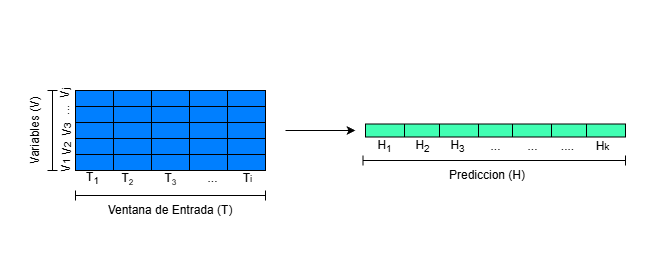
\includegraphics[width=0.85\textwidth]{Figuras/estModelo.drawio (1).png}
  \caption{Representación esquemática de la estructura de entrada $(T, V)$ y salida $(H)$ del modelo. 
  Cada muestra de entrada contiene $T$ días consecutivos de $V$ variables hidrometeorológicas, 
  y el modelo predice los valores del nivel del río para los próximos $H$ días.}
  \label{fig:estructura_datos}
\end{figure}

\begin{table}[h]
  \centering
  \caption{Ejemplo ilustrativo de una ventana de entrada con $T=5$ días y $V=3$ variables.}
  \label{tab:ejemplo_tensor}
  \begin{tabular}{c|ccc}
    \toprule
    \textbf{Día} & \textbf{Nivel (m)} & \textbf{Caudal (m$^3$/s)} & \textbf{Precipitación (mm)} \\
    \midrule
    $t-4$ & 3.22 & 1200 & 5.3 \\
    $t-3$ & 3.18 & 1100 & 1.2 \\
    $t-2$ & 3.05 & 980  & 0.0 \\
    $t-1$ & 2.98 & 970  & 0.8 \\
    $t$   & 2.95 & 950  & 0.0 \\
    \bottomrule
  \end{tabular}
\end{table}

\noindent
Esta formulación, ilustrada en la Figura~\ref{fig:estructura_datos} y detallada en la Ecuación~\eqref{eq:estructura_entrada_salida}, permite capturar dependencias temporales entre múltiples variables y facilita la comparación directa de distintos horizontes de predicción ($H$), sin necesidad de realizar iteraciones acumulativas paso a paso. La Tabla~\ref{tab:ejemplo_tensor} muestra cómo se organizan las observaciones dentro de una ventana temporal típica antes de ingresar al modelo.




\section{Partición y validación temporal}
\label{sec:particion_validacion}

La partición de los datos y la estrategia de validación se diseñaron para reflejar un escenario operativo realista y garantizar la generalización de los modelos:

\begin{enumerate}
  \item \textbf{Entrenamiento y validación inicial (1995–2012).}  
    \begin{itemize}
      \item Se emplearon todos los registros diarios entre el 01-01-1995 y el 31-12-2012. Durante el entrenamiento \texttt{validation\_split=0.2}, de modo que el 80\,\% de los registros se destinó a entrenamiento y el 20\,\% restante a validación.
      \item Esta partición 80–20 se empleó para ajustar hiperparámetros y prevenir sobre ajuste durante la fase inicial de entrenamiento.
    \end{itemize}


  \item \textbf{Conjunto de prueba independiente (2013–2022).}  
    \begin{itemize}
      \item Las observaciones diarias desde el 01-01-2013 hasta el 31-12-2022 se reservan como \emph{test}, sin usarse ni para entrenar ni para validar.  
      \item Este bloque de datos permite evaluar el desempeño de los modelos frente a información completamente “nueva”, simulando su uso en producción durante diez años completos.
    \end{itemize}

  \item \textbf{Validación temporal adicional y reentrenamiento anual (2013–2022).}  
    \begin{itemize}
      \item A partir de 2013, se adopta un esquema de \emph{reentrenamiento periódico} mediante ventanas móviles:
        \begin{itemize}
          \item Cada año, el modelo se reentrena usando todos los datos disponibles hasta el 31 de diciembre del año anterior.  
          \item Por ejemplo, para predecir en 2013, se usa el modelo entrenado sobre 1995–2012; para 2014, se recalibra con datos de 2013, y así sucesivamente hasta 2022.  
        \end{itemize}
      \item En cada ciclo de reentrenamiento, se reutilizan los pesos del modelo anterior, ajustando únicamente con el nuevo año de datos, lo que simula un entorno operacional donde el modelo se actualiza anualmente con la información más reciente.
    \end{itemize}
\end{enumerate}

Este enfoque mixto—split inicial 80–20, test independiente y reentrenamiento anual—asegura:
\begin{itemize}
  \item Un ajuste de hiperparámetros robusto sin “fugar” información futura.  
  \item Una evaluación del rendimiento sobre datos no vistos durante el entrenamiento.  
  \item Una validación continua de la capacidad del modelo para adaptarse a cambios hidrometeorológicos a lo largo de los años.
\end{itemize}

\section{Ajuste de hiperparámetros} \label{ssec:ajuste_hiperparametros}

El proceso de optimización del modelo se organizó en una serie de etapas sucesivas orientadas a mejorar progresivamente el desempeño del modelo base presentado en trabajos anteriores. A diferencia de dicho modelo, que se entrenaba una única vez sobre datos históricos, en esta propuesta se introduce un esquema de reentrenamiento periódico y adaptativo, además de una integración sistemática de variables exógenas. La biblioteca \textit{Optuna} se utilizó como marco de optimización bayesiana para explorar el espacio de configuraciones posibles, considerando múltiples métricas de evaluación (RMSE, MAE, MAPE y NSE), priorizando estas dos últimas para la selección final de los mejores ensayos.

\paragraph{Etapa 1: Optimización del esquema de reentrenamiento.}
En esta etapa inicial, se evaluaron diferentes frecuencias de tiempo para el reentrenamiento del modelo, utilizando intervalos que variaban entre 3 y 36 meses. El procedimiento consistió en entrenar inicialmente el modelo con todo el conjunto histórico disponible, exceptuando los últimos 10 años, y luego reentrenarlo, durante el período de tiempo exceptuado, de forma periódica sobre ventanas móviles del tamaño especificado. La búsqueda identificó que una frecuencia de reentrenamiento de 12 meses producía los mejores resultados, balanceando precisión y capacidad de adaptación.

\paragraph{Etapa 2: Incorporación secuencial de variables exógenas.}
Una vez establecido el esquema de reentrenamiento, se evaluó el impacto de diferentes grupos de variables hidrometeorológicas sobre el rendimiento del modelo. Este proceso se realizó de manera estructurada y progresiva, incorporando primeramente caudales, luego precipitaciones acumuladas, y finalmente ambas categorías en conjunto. Esta exploración permitió verificar empíricamente el valor predictivo de cada tipo de información adicional.

\paragraph{Etapa 3: Selección automática del conjunto óptimo de variables.}
Con base en los resultados previos, se realizó una búsqueda exhaustiva utilizando 3000 configuraciones distintas para identificar el conjunto más adecuado de variables de entrada. Esta búsqueda incluyó diferentes estaciones de medición de niveles, caudales y precipitaciones, así como la cantidad de días de acumulación para cada serie de precipitaciones. Se utilizaron acumulaciones entre 0 y 360 días, considerando combinaciones posibles de las estaciones no fijas. El conjunto óptimo seleccionado incluyó estaciones tanto de caudal como de precipitación acumulada con distintos niveles de acumulación, según se detalla en la Tabla~\ref{tab:variables_seleccionadas}.

\begin{table}[h]
  \centering
  \caption{Selección de variables y estaciones utilizadas en el modelo}
  \label{tab:variables_seleccionadas}
  \begin{tabular}{@{}ll@{}}
    \toprule
    \textbf{Elemento}                   & \textbf{Descripción}                                                                              \\ \midrule
    Estaciones base                     & Nivel: 86134, 86183, 86218.                                                                      \\
    Estaciones candidatas (Nivel)      & 86010, 86088.                                                                                   \\
    Estaciones candidatas (Caudal)     & 86218, 86134.                                                                                   \\
    Estaciones candidatas (Precipitación)& 86170, 86134, 86128.                                                                            \\ \midrule
    Estaciones seleccionadas (Nivel)    & 86134, 86183, 86218, 86088.                                                                      \\
    Estaciones seleccionadas (Caudal)   & 86218, 86134.                                                                                   \\
    Estaciones seleccionadas (Precipitación) & 86170, 86134, 86128.                                                                        \\
    Acumulaciones evaluadas (Precipitación)   & 0 a 360 días por estación                                                                    \\
    Acumulación óptima por estación    & 86170: 191 días, 86134: 2 días, 86128: 215 días.                                                 \\ \bottomrule
  \end{tabular}
\end{table}

\paragraph{Etapa 4: Optimización de hiperparámetros del modelo.}
Posteriormente, se ajustó los parámetros clave del modelo relacionados con su arquitectura y dinámica de entrenamiento. Estos incluyeron: la longitud de la ventana de entrada, la cantidad de unidades en la capa GRU, el tamaño de los lotes utilizados durante el entrenamiento, la tasa de abandono (dropout), el número de épocas, la tasa de aprendizaje inicial, los criterios de parada temprana, los factores de ajuste automático de la tasa de aprendizaje y el parámetro delta de la función de pérdida de Huber. Se realizaron 1000 búsquedas distintas para explorar el espacio combinado de estos valores. Los valores seleccionados se resumen en la Tabla~\ref{tab:hiperparametros_modelo}.

\begin{table}[h]
  \centering
  \caption{Rangos y valores óptimos: Hiperparámetros del modelo}
  \label{tab:hiperparametros_modelo}
  \begin{tabular}{@{}lll@{}}
    \toprule
    \textbf{Parámetro}                            & \textbf{Rango explorado}               & \textbf{Valor óptimo} \\ \midrule
    Ventana de entrada                            & 100 a 750 días                          & 257 días              \\
    Unidades en GRU                               & 16, 32, 64, 128, 256, 512               & 32                    \\
    Tasa de abandono (dropout)                    & 0.1 a 0.4                               & 0.318                 \\
    Tasa de aprendizaje inicial (log-escala)      & $10^{-5}$ a $10^{-1}$                   & 0.0062                \\
    Épocas (entrenamiento inicial)                & 10 a 100 (incrementos de 10)            & 50                    \\
    Tamaño de lote                                 & 8, 16, 32, 64, 128                      & 8                     \\
    Parada temprana (paciencia)                   & 3 a 20                                  & 12                    \\
    Parada temprana (inicio)                      & 5 a 20                                  & 6                     \\
    Factor del scheduler                           & 0.1 a 0.9 (incrementos de 0.1)          & 0.1                   \\
    Paciencia del scheduler                        & 3 a 15                                  & 7                     \\
    Tasa mínima del scheduler (log-escala)         & $10^{-6}$ a $10^{-4}$                   & $1.61 \times 10^{-5}$ \\
    Delta de Huber ($\delta$)                      & $10^{-2}$ a $10^{2}$ (log-escala)        & 0.0197                \\ \bottomrule
  \end{tabular}
\end{table}

\paragraph{Etapa 5: Optimización específica del proceso de reentrenamiento.}
Finalmente, se realizó una etapa adicional de optimización centrada exclusivamente en los parámetros utilizados durante los ciclos de reentrenamiento anual. Entre los aspectos ajustados se incluyeron la tasa de aprendizaje para el reentrenamiento, la cantidad de épocas y el tamaño de lote empleado en esta fase. Esta búsqueda se realizó sobre 150 configuraciones distintas cuyos resultados óptimos se presentan en la Tabla~\ref{tab:hiperparametros_reentreno}.

\begin{table}[h]
  \centering
  \caption{Rangos y valores óptimos: Reentrenamiento y configuración operativa}
  \label{tab:hiperparametros_reentreno}
  \begin{tabular}{@{}lll@{}}
    \toprule
    \textbf{Parámetro}                                & \textbf{Rango explorado}          & \textbf{Valor óptimo} \\ \midrule
    Frecuencia de reentrenamiento                      & 3 a 36 meses                        & 12 meses              \\
    Tasa de aprendizaje (reentrenamiento) (log-escala) & $10^{-5}$ a $10^{-1}$               & $1.67 \times 10^{-5}$ \\
    Épocas (reentrenamiento)                           & 10 a 100                            & 90                    \\
    Tamaño de lote (reentrenamiento)                    & 8, 16, 32, 64, 128                  & 16                    \\ \bottomrule
  \end{tabular}
\end{table}


\section{Diseño de los experimentos} \label{sec:diseno_experimentos}

\subsection{Entrenamiento inicial}
El modelo fue entrenado inicialmente utilizando datos históricos del período 1995–2012, correspondientes a la estación objetivo (86218) y a las covariables seleccionadas en la Tabla~\ref{tab:variables_seleccionadas}. Este conjunto fue dividido en dos subconjuntos temporales:
\begin{itemize}
  \item \emph{80\,\% para entrenamiento}: registros desde el 01-01-1995 hasta el 31-12-2008.
  \item \emph{20\,\% para validación}: registros desde el 01-01-2009 hasta el 31-12-2012.
\end{itemize}
Durante esta fase, se emplearon los hiperparámetros óptimos definidos en las Tablas~\ref{tab:hiperparametros_modelo} y \ref{tab:hiperparametros_reentreno}, y se utilizó validación temprana (\textit{early stopping}) con paciencia de 12 épocas y comienzo de parada temprana en la época 6, basándose en la métrica de validación (Huber loss). El objetivo fue capturar patrones hidroclimáticos de largo plazo, incluyendo estacionalidades y tendencias estructurales del sistema.

\subsection{Reentrenamiento anual con ventana móvil}
A partir del año 2013, se implementó un esquema de reentrenamiento anual mediante una ventana móvil que simula un escenario operacional real. Por cada año $a$ en el rango 2013–2022:
\begin{enumerate}
  \item Se reutilizan los pesos del modelo entrenado hasta $a-1$ (inicialmente, el modelo de 1995–2012).
  \item Se reentrena durante las épocas definidas (90) utilizando únicamente los registros del año anterior completo ($a-1$).
  \item Se generan predicciones para los siguientes 28 días de cada día del año $a$, acumulando así un histórico de predicciones para todo el período 2013–2022.
\end{enumerate}
Este proceso permite evaluar la capacidad de adaptación del modelo frente a cambios hidrometeorológicos interanuales, manteniendo la consistencia operativa en la actualización de pesos mediante la tasa de aprendizaje y el tamaño de lote optimizados para reentrenamiento.

\subsection{Evaluación en conjunto de prueba (2013–2022)}
Las predicciones generadas para cada día del período 2013–2022 con horizonte de 28 días formaron el \emph{conjunto de prueba independiente}, ya que dichos datos no fueron utilizados durante el entrenamiento inicial ni en ningún reentrenamiento previo. Para cada predicción diaria se compararon los valores pronosticados contra los valores reales observados, calculando las métricas detalladas en la sección siguiente. Finalmente, se recopilaron las métricas globales y anuales a lo largo del decenio 2013–2022, permitiendo una evaluación robusta y acumulada del desempeño del modelo propuesto frente al modelo base.

\section{Métricas de evaluación} \label{sec:metricas_evaluacion}

Para cuantificar el desempeño predictivo del modelo en los horizontes de 1 a 28 días, se emplearon cuatro métricas estándar en estudios hidrológicos: NSE, RMSE, MAE y MAPE. Todas las métricas relacionadas al error se expresan en metros, excepto el MAPE que se reporta en porcentaje.

\subsection{Eficiencia de Nash–Sutcliffe (NSE)}
Se define como
\[
\text{NSE} \;=\; 1 \;-\; \frac{\displaystyle \sum_{i=1}^n \bigl(O_i - P_i\bigr)^2}{\displaystyle \sum_{i=1}^n \bigl(O_i - \overline{O}\bigr)^2},
\]
donde $O_i$ son los valores observados, $P_i$ los valores predichos, y $\overline{O}$ la media de los valores observados. Un valor de NSE cercano a 1 indica alta precisión, mientras que valores negativos reflejan que el modelo es menos efectivo que una predicción constante igual al promedio de la serie observada.

\subsection{Error cuadrático medio (RMSE)}
Se calcula como
\[
\text{RMSE} \;=\; \sqrt{\frac{1}{n} \sum_{i=1}^n \bigl(O_i - P_i\bigr)^2}.
\]
Cuanto menor sea el RMSE, mejor será el desempeño del modelo, dado que mide la magnitud promedio de los errores en las unidades de la variable (metros).

\subsection{Error absoluto medio (MAE)}
Se define como
\[
\text{MAE} \;=\; \frac{1}{n} \sum_{i=1}^n \bigl\lvert O_i - P_i \bigr\rvert.
\]
El MAE cuantifica la desviación promedio en valor absoluto entre observaciones y predicciones. Es menos sensible a valores atípicos que el RMSE.

\subsection{Error porcentual absoluto medio (MAPE)}
Se expresa en términos relativos:
\[
\text{MAPE} \;=\; \frac{100}{n} \sum_{i=1}^n \left\lvert \frac{O_i - P_i}{O_i} \right\rvert \times 100\%.
\]
El MAPE es especialmente útil para interpretar el error en porcentaje con relación a los valores reales, aunque debe manejarse con cuidado cuando las observaciones se acercan a cero.

Las métricas fueron calculadas sobre el total de predicciones generadas entre 2013 y 2022, así como de forma individual para cada año, permitiendo comparar el desempeño acumulado y la estabilidad interanual del modelo propuesto frente al modelo base.